\begin{center}
	\section{Dise\~no te\'orico} \label{teorico:sed}
\end{center}

\noindent
\justify

En la etapa de eluci\'on y filtrado de la planta de extracci\'on se busca separar la fase s\'olida de la l\'iquida. El dise\~no te\'orico de este sistema se desarrolla con base en lo estipulado en la secci\'on \ref{simplificado}, teniendo en cuenta las cosideraciones estipuladas en el Cuadro \ref{condiciones}.

\begin{table}[h!]
	\centering
	\begin{tabular}{c|p{4cm}}
		\hline
		\textbf{Par\'ametro} & \textbf{Valor} \\ \hline
		Cantidad de material s\'olido a remover $[kg]$ & 80 \\ \hline
		Densidad media del material s\'olido $\left[kg / m^3 \right]$ & 1700 \\ \hline
		Volumen de la mezcla $[L]$ & 200 \\ \hline
		Tama\~no de part\'icula medio $[\mu m]$ & 250 \\ \hline
		Tipo de solvente & Mezcla agua - etanol ($50 \%$) \\ \hline
		Temperatura del proceso $[\degree C]$ & 28 \\ \hline
		Tiempo del proceso $[h]$ & 1 \\ \hline
	\end{tabular}
	\caption{Condiciones operacionales.}
	\label{condiciones}
\end{table}

\noindent
\justify

El principio f\'isico de separaci\'on de sustancias empleado por el sistema es la \textbf{sedimentaci\'on}, producida por la diferencia de densidades entre el material s\'olido a separar y el solvente. Es debido a ello que en el presente trabajo se desarrolla el dise\~no y simulaci\'on num\'erica de un sedimentador de placas paralelas como sistema de eluci\'on y filtrado de la planta de extracci\'on.

\noindent
\justify

Para definir la geometr\'ia del sistema, se parte de las siguientes afirmaciones y suposiciones:

\begin{itemize}
	\item El fen\'omeno a describir se basa en la \textit{sedimentaci\'on discreta}; indicativo de que las part\'iculas no tienden a aglomerarse y se desprecian los efectos de colisi\'on entre ellas. 
	\item Cada part\'icula se trata como un cuerpo esf\'erico microm\'etrico de tama\~no equivalente a $250 [\mu m]$.
\end{itemize}

\subsection{Propiedades termodin\'amicas}

\noindent
\justify

Para desarrollar la automatizaci\'on del dise\~no, es necesario predecir el valor de las propiedades del solvente a cualquier valor de temperatura y relaci\'on agua - etanol. Para ello, se inicia calculando las propiedades del etanol y del agua a presi\'on atmosf\'erica empleando las Ecuaciones \ref{rhoH2O}. \ref{viscH2O}, \ref{rhoEt} y \ref{viscEt}.

\begin{equation}
	\rho _{H_2O} = 1.00048675 \, 10^3 - 2.23243162 \, 10^{-2}*T - 4.60579811 \, 10^{-3}*T^2 \equiv \left[ kg / m^3 \right] 
	\label{rhoH2O}
\end{equation}

\begin{equation}
	\mu _{H_2O} = 1.63190407 \, 10^{-6} - 3.73507082 \, 10^{-8}*T + 3.20602877 \, 10^{-10}*T^2 \equiv \left[ m^2 / s \right] 
	\label{viscH2O}
\end{equation}


\begin{equation}
	\rho _{et} = 8.06320738 \, 10^{2}-8.32481402 \, 10^{-1}*T-5.78205398 \, 10^{-4}*T^2 \equiv \left[ kg / m^3 \right] 
	\label{rhoEt}
\end{equation}

\begin{equation}
	\mu _{et} = 2.11316694 \, 10^{-6} - 3.69955667 \, 10^{-8}*T + 2.57275555 \, 10^{-10}*T^2 \equiv \left[ m^2 / s \right] 
	\label{viscEt}
\end{equation}

\noindent
\justify

Una vez conocidas las propiedades individuales, se calcula la propiedad de la mezcla a trav\'es de la Ecuaci\'on \ref{mezcla}.

\begin{equation}
	\lambda _f = (1-x) \, \lambda _{H_2O} + x \, \lambda _{et}
	\label{mezcla}
\end{equation}

\noindent
\justify

D\'onde: $\lambda$ es la propiedad termodin\'amica (densidad, viscosidad, etc) $x$ es la concentraci\'on de la mezcla.

\noindent
\justify

Para las condiciones dadas en el Cuadro \ref{condiciones}, las propiedades termodin\'amicas de la mezcla se pueden apreciar en el Cuadro \ref{temoM}.

\begin{table}[h!]
	\centering
	\begin{tabular}{|c|c|}
	\hline
	\textbf{Propiedad} & \textbf{Valor} \\ \hline
	$\rho _f \left[ kg / m^3 \right]$ & $889.4$ \\ \hline
	$\mu _f \left[ m^2 / s \right] $ & $1.06 \, 10^{-6}$ \\ \hline
	\end{tabular}
	\caption{Propiedades de la mezcla agua - etanol al $50 \%$.}
	\label{temoM}
\end{table}

\subsection{Naturaleza del flujo}

\noindent
\justify

Para asegurar el \'exito del sistema de sedimentaci\'on, el flujo dentro del sistema no puede ser de car\'acter turbulento. Debido a ello, seg\'un Miguel Vire (\textit{"Dise\~no de la planta de potabilizaci\'on del agua"}), se asume regimen laminar; cuya velocidad de flujo se determina a trav\'es de la Ecuaci\'on \ref{V_lam}.

\begin{equation}
	V_{laminar} = \frac{g}{18} \, (S_s - 1) \, \left(\frac{d_{particula}^2}{\mu} \right)
	\label{V_lam}
\end{equation}

\noindent
\justify

D\'onde: $V_{laminar}$ es la velocidad del flujo laminar, $S_s$ es una constante, $d_{particula}$ es el di\'ametro de una part\'icula y $\mu$ es el valor de la viscosidad cinem\'atica del fluido.

\noindent
\justify

El n\'umero de Reynolds caracteriza la naturaleza de un flujo y se calcula con base en la siguiente relaci\'on matem\'atica.

\begin{equation}
	Re = \frac{V_{laminar} \, d_{particula}}{\mu}
	\label{Re}
\end{equation}

\noindent
\justify

Con base en la Ecuaci\'on \ref{Re}, el n\'umero de Reynolds tiene un valor de $3.625$; valor superior a $1.0$ e inferior a $1000$. Indicativo de que el flujo no es de car\'acter laminar ni turbulento, encontr\'andose en el \textbf{r\'egimen de transici\'on}.

\subsection{Par\'ametros operacionales}

\noindent
\justify

Al encontrarse el flujo en r\'egimen de transici\'on, la velocidad de flujo se calcula a aprtir de la Ley de Allen, mostrada en la Ecuaci\'on \ref{V_trans}.

\begin{equation}
	V_{transicion} = 36 \sqrt{(S_s-1) \, \frac{d_{particula}}{C_D}}
	\label{V_trans}
\end{equation}


\noindent
\justify

En donde $C_D$ es una constante que se calcula de la siguiente forma:

\begin{equation}
	C_D = \frac{24}{R_{corregio}} + \frac{3}{\sqrt{Re_{corregido}}} + 0.34
	\label{C_D}
\end{equation}

\noindent
\justify

A partir de las caracter\'isticas de las part\'iculas y del agua, se obtienen las constantes $K_1$ y $K_2$ de la Figura \ref{G1}; en donde $X_1 = K_1  \, d$. De modo que:

\begin{equation*}
	\left( \frac{g \, (S_s-1)}{\mu ^2} \right) ^{1/3} = K_1
\end{equation*}

\begin{equation*}
	\left[ g (S_s-1) \mu \right] ^{1/3} = K_2
\end{equation*} 

\begin{figure}[h!]
	\centering
	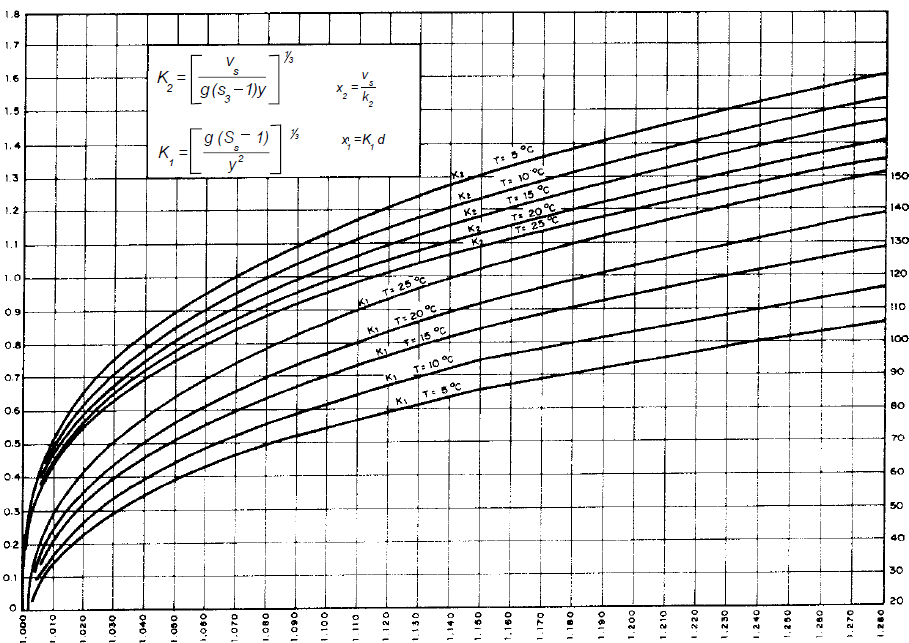
\includegraphics[width=0.8\textwidth]{Images/Sedimentacion/G1.PNG}
	\caption{Velocidad de asentamiento de part\'iculas discretas en un fluido est\'atico.}
	\label{G1}
\end{figure}

\noindent
\justify

Se calcula una velocidad de transici\'on \textit{corregida} para la determinaci\'on del n\'umero de Reynolds que se calcula de la siguiente forma:

\begin{equation*}
	V_{corregida} = X_2 \, K_2
\end{equation*}

\begin{equation}
	Re_{trans} = \frac{V_{corregida} \, d_{particula}}{\mu}
\end{equation}

\noindent
\justify

El n\'umero de Reynolds de transici\'on presenta un valor de $2.858$ con una velocidad de $1.446 [cm/s]$.

\subsection{Dimensionamiento}

\noindent
\justify

El sistema de filtrado se trata de un equipo sedimentador de placas planas paralelas inclinadas a $60 \degree$. La velocidad cr\'itica de sedimentaci\'on de las part\'iculas se calcula a partir de la Ecuaci\'on \ref{yao} (f\'ormula de Yao), la cual define el valor de la velocidad m\'inima requerida para que una part\'icula se sedimente. 

\begin{equation}
	V_{sc} = \frac{S_c \, V_0}{\sin \theta + L_{rel} \cos \theta}
	\label{yao}
\end{equation}

\noindent
\justify

De la Ecuaci\'on \ref{yao}, $S_c$ es una constante de sedimentaci\'on cuyo valor es $1$ para sistemas de \textit{placas paralelas}, $V_0$ es la magnitud de la velocidad del flujo, $L_{rel}$ es la relaci\'on entre la longitud de una lamela y el ancho de la misma; y $\theta$ es el \'angulo de inclinaci\'on de las placas.

\noindent
\justify

La relaci\'on entre el ancho $e$ del conducto y la longitud $L$ tiene una importancia especial en la eficiencia del sedimentador. Si esta relaci\'on $L_{rel}$ es muy peque\~na, cada sedimentador act\'ua como un sedimentador horizontal corriente de baja velocidad. Debido a que la eficiencia var\'ia lentamente para una $L_{rel} > 20$, se toma un valor de $20$.

\noindent
\justify

Para que un sedimentador pueda trabajar con alta velocidad, es necesario que exista flujo laminar en las celdas, esto es que el n\'umero de Reynolds sea inferior a 250. Cualquier turbulencia puede generar arrastre de part\'iculas, bajando notoramiente la eficiencia; raz\'on por la que se emplea como criterio principal de dise\~no. 

\begin{equation}
	N_R = \frac{V_0 \, 4 R_h}{\mu}
	\label{Reynolds}
\end{equation}

\noindent
\justify

En d\'onde $R_h$ es el radio hidr\'aulico, cuyo valor est\'a definido por la Ecuaci\'on \ref{Rh}.

\begin{equation}
	R_h = \frac{b \, e}{2(b+e)}
	\label{Rh}
\end{equation}

\noindent
\justify

De la Ecuaci\'on \ref{Rh}: $b$ es el ancho de la lamela y $e$ el largo de la misma. Dimensiones que definen el \'area transversal de una lamela. 

\noindent
\justify

A partir de un proceso iterativo, se obtuvo que las mejores dimensiones son: $b = 30 [cm]$ y $e = 2 [cm]$; lo que se traduce en un n\'umero de Reynolds de $89.69$ (r\'egimen laminar).

\subsubsection{Panel de lamelas}

\noindent
\justify

La mejor relaci\'on de eficiancia referente al n\'umero de lamelas est\'a entre 5 y 8 lamelas, por lo que se escoge desarrollar el proceso de dise\~no con 6 lamelas en el panel; seleccionando l\'aminas de calibre 24 para su construcci\'on.

\noindent
\justify

El distanciamiento horizontal entre lamelas se calcula de la siguiente forma:

\begin{equation}
	e_x = \frac{e}{\sin \theta}
\end{equation}

\noindent
\justify

Obteniendo un distanciamiento de $2.31 [cm]$. El ancho total del panel se puede calcular a trav\'es de la Ecuaci\'on \ref{anchoP}.

\begin{equation}
	P_{ancho} = e_x (N_{lamelas}-1) + t_{lamela} \, N_{lamelas} + L_{lamela} \cos \theta \rightarrow P_{ancho} = 34.68 [cm]
	\label{anchoP}
\end{equation}

\noindent
\justify

El alto del panel se calcula de la siguiente forma:

\begin{equation}
	P_{alto} = L_{lamela} \sin \theta \rightarrow P_{alto} = 39.45 [cm]
\end{equation}

\noindent
\justify

La profundidad del panel es equivalente al ancho de la lamela: $30 [cm]$.


\subsection{M\'etodo de Hazen $\rightarrow$ tiempo de sedimentaci\'on}

\noindent
\justify

El concepto de carga hidr\'aulica superficial (par\'ametro de Hazen) compara la velocidad de sedimentaci\'on de la part\'icula para conocer si alcanza a sedimentarse durante el trayecto por el sistema. La \textit{altura} de sedimentaci\'on requerida se calcula mediante la Ecuaci\'on \ref{Hsed}.

\begin{equation}
	H_{sedimentacion} = \frac{e}{\cos \theta}
	\label{Hsed}
\end{equation} 

\noindent
\justify

La altura de sedimentaci\'on requerida es de $4 [cm]$ (distanciamiento vertical entre lamelas), cuyo tiempo de sedimentaci\'on se calcula a trav\'es de la siguiente relaci\'on matem\'atica:

\begin{equation}
	t_{sed} = \frac{H_{sedimentacion}}{V_{corregida}}
	\label{tsed}
\end{equation}

\noindent
\justify

De acuerdo a la Ecuaci\'on \ref{tsed}, se requieren de $2.767 [s]$ para sedimentar las part\'iculas dentro de cada celda.

\subsection{Tama\~no de part\'icula m\'inima}

\noindent
\justify

El tama\~no de part\'icula \textit{m\'inima} se calcula a trav\'es de la Ecuaci\'on \ref{d_par}.

\begin{equation}
	V_{sc} = 0.22 \left[g \left( \frac{\rho _{solido} - \rho _{fluido}}{\rho _{fluido}} \right) \right] ^{2/3} \frac{d_{particula}}{\sqrt[3]{\frac{\mu}{\rho _{fluido}}}}
	\label{d_par}
\end{equation}

\noindent
\justify

De esta manera, se concluye que el sistema dise\~nado est\'a capacitado para retirar part\'iculas de hasta $40 [\mu m]$. La eficiencia del sistema se calcula a trav\'es de la siguiente relaci\'on matem\'atica:

\begin{equation}
	Ef = 1 - \frac{V_{sc}}{V_0}
\end{equation} 

\noindent
\justify

Obteniendo un valor cercano al $91 \%$.

\newpage

\subsection{Resultados}

\noindent
\justify

En resumen, los resultados del proceso de dise\~no funcional del sistema se pueden apreciar en el Cuadro \ref{resul_dis}.

\begin{table}[h!]
	\centering
	\begin{tabular}{c|c}
		\hline
		\textbf{Par\'ametro} & \textbf{Valor} \\ \hline
		Caudal $\left[m^3 /h \right]$ & $0.3$ \\ \hline
		Tiempo $[h]$ & $1$ \\ \hline
		Altura lamela $[cm]$ & $20$ \\ \hline
		Ancho lamela $[cm]$ & $2.5$ \\ \hline
		\'Angulo de inclinaci\'on $[\degree ]$ & 60 \\ \hline
		Ancho panel $[cm]$ & $25$ \\ \hline
		Tama\~no de part\'icula m\'inima $[\mu m]$ & 40 \\ \hline
		Tama\~no de part\'icula media $[\mu m]$ & 250 \\ \hline
		Eficiencia general del sistema & $91 \%$ \\ \hline
	\end{tabular}
	\caption{Resumen de resultados.}
	\label{resul_dis}
\end{table}

\noindent
\justify

Estos resultados definen la geometr\'ia para el desarrollo de las simulaciones num\'ericas CFD y CFD-DEM en el cap\'itulo \ref{CFD-DEM}.